\chapter{Funktionale Programmierung (Scheme)}
Scheme folgt dem deklarativ-funktionalem Programmierparadigma. Nachfolgend einige Beispiele von funktionale Programmiersprachen: LISP (Common Lisp, Scheme, Clojure), MetaLanguage (ML) Familie (SML, OCaml, F\#) und Haskell.

LISP (LISt Processing) ist durch das Lambda Kalkül inspiriert und ist homoikonisch. Homoikonizität bedeutet Selbst-Abbildbarkeit oder Selbst-Repräsentiertbarkeit. Dies ist eine Eigenschaft von Programmiersprachen, dass Programme gleichzeitig Datenstrukturen derselben Sprachen sind. In solchen Sprachen ist es einfach Programme zu schreiben, die Programme schreiben (Turingmaschine). (In LISP ist jedes Programm eine Liste)

\section{Prinzipien der funktionalen Programmierung}
Im Zentrum stehen Funktionen und die Anwendung von Funktionen:
\begin{itemize}
	\item Rekursion statt Schleifen
	\item Keine Seiteneffekte (referentielle Transparenz)
	\item Funktion als gleichberechtigte Datenobjekte
	\item Verwendung von einer Funktions-Implementierung für verschiedene Typen (Polymorphismus)
	\item Programme sind kürzer, klarer, besser zu warten, zuverlässiger, schneller zu erstellen
\end{itemize}
Aufgaben werden in kleinere Aufgaben zerlegt (Dekomposition) um diese schlussendlich wieder zusammenzuführen (Komposition).

\section{DrRacket}
DrRacket ist eine integrierte Entwicklungsumgebung (IDE) für den Scheme-Dialekt Racket. Es können verschiedene, skalierbare Scheme-Dialekte ausgeführt werden. Hat eine REPL Konsole (Read-Evalute-Print Loop) integriert. Zudem gibt es einen Stepper bei dem der Funktionsaufruf verfolgt werden kann.

\section{Syntax}
\begin{description}
	\item[Zahlen] Primitive atomare Ausdrücke. Nebst rationalen Zahlen können auch reelle, irrationale und komplexe Zahlen definiert werden.
	\item[Bool] Es gibt true und false. Alternative Darstellungen: \#t, \#f, \#true, \#false.
	\item[Operatoren] Scheme hat eingbaute mathematische Operatoren, welche auch als PRIMS-OPS (primitve operations) bezeichnet werden. Beispiele: +, -, *, /, quotient, remainder, expt, modulo, abs, max, min, sin, tan, exp ...
	\item[Form] Fast alles in folgender Form deklariert werden: \emph{(<operator> <operand1> <operand2> ...)}. Dabei ist die Reihenfolge der Auswertung nicht festgelegt! Wichtig: Diese Notation nennt man \textbf{Form}! Formen werden ausgewertet.
	\item[Klammern] Die Klammern sind Fluch und Segen zugleich. Die Operatorrangfolge kann selbst definiert werden. Nachteil: Hohe Zahl der Klammern. Gewisse Scheme-Implementation wie Racket unterstützen auch eckige Klammern. Man erhält etwas mehr Übersicht.
\end{description}

\begin{lstlisting}[caption=Simple mathematische Operationen]
> (+ 13 52)
65
> (- 26 33)
-7
> (/ 5 10)
0.5
> (* 13 5)
65
> (* 5 2 3)
30
> (/ 10 2 5)
1
> (+ 1 (* 2 8) (* 4 4) (* 8 2) (* 1 16))
65
\end{lstlisting}

\section{Auswertungsregeln}
Es ist klar, dass Zahlen und boolsche Werte selbst auswertend sind und ihren Wert zurückgegeben. Ein Name gibt den Wert zurück mit welchem dieser in der Umgebung assoziiert ist. Die eingebauten Operatoren geben die Sequenz an Instruktionen zurück.
Wenn die Dinge kombiniert werden, dann wird rekursiv ausgewertet. Es werden alle Unterausdrücke in \emph{beliebiger} Form ausgewertet. Wichtig zu wissen ist, dass nicht definiert ist, welcher Operand pro Form in welcher Reihenfolge ausgewertet ist. Also nicht links nach rechts wie bspw. in Java.

\subsection{Funktions-Auswertung}
Bei einer \textbf{strikten Auswertung} werden alle Argumente zuerst ausgewertet bevor die Funktion aufgerufen wird (Scheme). Eine andere Möglichkeit wäre die \textbf{lazy evaluation}, wobei die unausgewerteten Ausdrücke übergeben werden. Die Auswertung erst dann, wenn die Werte benötigt werden.

\newpage
\section{Namen definieren}
\begin{lstlisting}[caption=Namen definieren]
(define <identifier> <expression>)
% <identifier> Beliebiger Name auch Sonderzeichen. Per Default case-sensitive, in DrRacket ausschaltbar.
% <expression> Beliebiger Ausdruck - Konstante, Variable, Funktionsaufruf, ...

> (define pi 3.14159)
pi: this name was defined previously and cannot be redefined - pi bereits eine Scheme Konstante
> (define PI 3.14159)

% Define wird speziell ausgewertet. Dabei wird der zweite Ausdruck nicht ausgewertet (im Beispiel pi). Zudem ist der Rückgabewerte von define nicht spezifiziert.
\end{lstlisting}

\section{Funktionen}
Beim Aufruf von Funktionen müssen die aktuellen Parameter in Anzahl, Datentyp (implizit) und Reihenfolge mit den formalen Parameter übereinstimmen. Es gibt keine Start-Funktion (kein main).

\begin{figure}[h!]
\centering
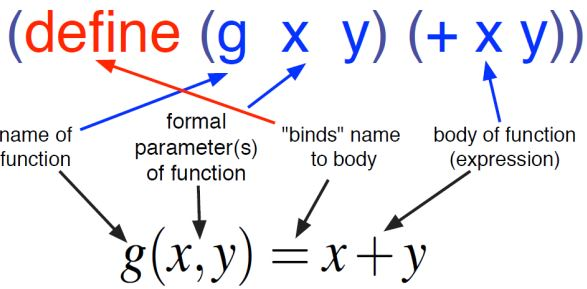
\includegraphics[width=0.5\linewidth]{fig/scheme-function-definition}
\caption{Scheme: Funktionen definieren}
\label{fig:scheme-function-definition}
\end{figure}

\begin{lstlisting}[caption=Beispiel Funktionen]
(define (area-of-disk r) (* PI (sqr r)))

> (area-of-disk 5)
78.53975

> (- (area-of-disk 5) (area-of-disk 3))
50.26544

(define (area-of-ring outer inner)
	(- (area-of-disk outer) (area-of-disk inner)))

> (area-of-ring 5 3)
50.264
\end{lstlisting}

\section{Funktionale Modellierung}
Ein OO-Entwickler muss nun etwas anders denken. Es gibt quasi immer eine Hauptfunktion, welche Hilfsfunktionen für Teilberechnungen nutzt. Hierarchisches Denken ist dabei gefordert.

\section{Prädikate}
True und false sind elementare Prädikate. Ein Prädikat ist ein Ausdruck der zu true oder false evaluiert. Wie Vergleichsoperatoren und boolesche Verknüpfungen.
\begin{lstlisting}[caption=Prädikate]
> (< 3 1)
false
> (<= 5 5)
true
>(<= 3 4 5 5)
true
> (< 3 4 5 5)
false

% AND-Verknüpfungen werden von links nach rechts ausgwertet. Evaluiert ein Ausdruck links zu false, dann wird die Auswertung beendet. Falls ein Ausdruck keinen boolschen Wert zurückgibt, kommt es zum Laufzeitfehler.
> (and (= 23.3 23.3) (< 5 7))
true
> (and true (+ 3 5))
and: question result is not true or false: 8

> (define x 0)
> (and (not (= x 0)) (< (/ 1 x) 1))
false

% OR-Verknüpfungen werden nur bis zum ersten true ausgwertet.
> (or (= 23.3 23.3) (< 5 7))
true

% Boolesche Vergleiche müssen so gemacht werden, der = Operator ist nur für Zahlen
(boolean=? <expr1> <expr2>)
\end{lstlisting}

\subsection{Prädikatsfunktionen}
Diese liefern immer einen Wahrheitswert zurück. Der Funktionsname endet mit einem Fragezeichen.
\begin{description}
	\item[Test auf Zahlen] integer? real? rational? complex? odd? even? zero? negative? positive?
	\item[Test auf Basistypen] boolean? number? char? null? string? symbol? procedure?
	\item[Test auf Gleichheit] string=? null=? equal? eq? eqv? char=?
\end{description}

\begin{lstlisting}[caption=Prädikatsfunktionen]
> (string? "Hallo ?")
true
> (string? "333")
true
> (string? 333)
false
> (number? 333)
true
> (number? "333")
false
\end{lstlisting}

Es können eigene Prädikate definiert werden \emph{(define <identifier?> <expression>)}. Das Fragezeichen muss angehängt werden. Ausserdem muss diese einen booleschen Wert zurückliefern.

\section{Symbole}
Nebst Zahlen und booleschen Werten gibt es Symbole. Symbole sind eine Sequenz von Zeichen angeführt von einem einfachen Anführungszeichen. Es gibt nur eine Operation auf diesem Datentyp \emph{symbol=?}. Symbole sind atomar und können nicht zerlegt werden. Im Gegensatz zu Strings werden sind keine Manipulationen möglich, der Vergleich ist sehr effizient und haben gewisse Einschränkung in der Zeichenwahl.

\begin{lstlisting}[caption=Symbole]
> (symbol=? 'Hallo 'Hallo)
true
> (symbol=? 'Hallo 'ABC)
false
> (symbol=? 1 2)
symbol=?: expects a symbol as 1st argument, given 1
\end{lstlisting}

\section{Fallunterscheidung}
Mittels \emph{cond} können Fallunterscheidungen realisiert werden. Es dürfen beliebig viele Klausen verwendet werden und die letzte Klause \emph{else} ist optional. Die Klauseln müssen in Klammern eingeschlossen sein. Die Abarbeitung ist von oben nach unten (Reihenfolge wichtig). Achtung: Wenn kein Fall zu true auswertet, gibt es einen Laufzeitfehler. Wenn \emph{else} nicht weggelassen wird, passiert das nie, den \emph{else} ist immer \emph{true}. 

\begin{lstlisting}[caption=Fallunterscheidung]
(cond (<cond clause1> <expr1>)
	(<cond clause2> <expr2>)
	...
	(else <last-expr>))
	
(define (grade score)
	(cond
		((not (number? score)) "Zahl eingeben!")
		((not (integer? score))
			"Ganze Zahl 0 <= x <= 15 eingeben!")
		((<= 13 score 15) "ausgezeichnet")
		((<= 10 score 12) "sehr gut")
		((<= 7 score 9) "gut")
		((<= 4 score 6) "ausreichend")
		((<= 1 score 3) "nicht erfüllt: Nachbesserung")
		((= 0 score) "nicht erfüllt")
		(else "Ganze Zahl 0 <= x <= 15 eingeben!")
	)
)
\end{lstlisting}

\newpage
\section{Selektion}
Mittels \emph{if} können Selektionen realisiert werden. Der \emph{else}-Teil ist nicht optional. \emph{cond} und \emph{if} sind gleichmächtig. Die eine Form kann in die andere Form transformiert werden.

\begin{lstlisting}[caption=Selektion]
(if (<test>) <then-expr> <else-expr>)

# Speziell: if verwendet nicht die strikte Auswertung, sondern die lazy evaluation.

(define (test a b)
	(if (= a 0) 1 b))
	
> (test 0 (/ 1 0))
/: division by zero	

# Und nun if selber:
>(if (= 0 0) 1 (/ 1 0))
1
\end{lstlisting}

\section{Datentyp: Struktur}

\begin{lstlisting}[caption=Strukturen]
# Definition
(define-struct <typename> (<field1> ... <fieldN>))

# Durch die Defintion von Strukturen, kommen drei weitere Typen von Funktionen mit

# Konstruktor (sind selbstauswertend)
(make-<typename> <value1>...<valueN>)

# Prädikatsfunkion
(<typename>? <objekt>)

# Feld-Selektor für jedes Feld
(<typename>-<field> <objekt>)

# Der Variable gibt man schlauerweise noch einen Namen
(define <name> (make-<typename> <value1>...<valueN>))

# Beispiele
(define-struct member (lastname firstname number))
(define-struct point (x y)) ; Typ-Definition
(make-point 7 3) ; Konstruktor-Aufruf
(define p1 (make-point 3 4)) ; Variablen-Definition

> (point? p1)
#true
> (point-x p1)
3
> (point-y p1)
4 >

# P.S.: Es können keine Typendefintionen definiert werden. In Scheme kommentiert man die Datentypen in den Strukturen.

# Scheme hat einen vordefinierte Struktur für den Punkt: posn (x y)
\end{lstlisting}

\section{Listen}
Das Problem von Strukturen ist, dass nur eine feste Zahl von Daten gespeichert werden können. Wir benötigen Listen. Die Elemente in \textbf{rekursiven Datenstrukturen} können Elemente der selben Datenstruktur beinhalten. Ein\textbf{Rekursionsanker} (Rekursionbasis) wird benötigt, um eine endliche Datenstruktur zu bekommen.
Die Definition einer Liste in Scheme ist rekursiv. Eine Liste ist leer oder besteht aus dem ersten Element und den Rest, welche wiederum eine Liste ist. Listen können beliebige Datentypen enthalten (Mischung möglich). Zudem können sie auch beliebig verschachtelt sein.

\begin{lstlisting}[caption=Listen]
% Konstruktor. Argument 1: Element, Argument 2: Liste.
(cons <element> empty)
(cons <element> (cons ... (cons <element> empty)))

> (cons "Bob" (cons "Tom" (cons "John" empty)))
(list "Bob" "Tom" "John")

% List statt cons (handlicher) (wertet Argumente aus)
(list <element1> ... <elementN>)

> (list 1 2 3)
(list 1 2 3)
> (list (list 'a 1) (list 'b 2))
(list (list 'a 1) (list 'b 2))

% Quote statt list (noch handlicher) (wertet Argument nicht aus)
'(1 2 3) % ist die Kurzform für (list 1 2 3)
'((1 2) (3 4) (5 6)) % steht für (list (list 1 2) (list 3 4) (list 5 6))
'(a b c) % steht für (list 'a 'b 'c)

% Listen Funktionen
empty % Leere Liste

(first <list>) % Selektor für das erste Element (früher car - IBM Relikt)

(rest <list>) % Selektor für den Rest (früher cdr - IBM Relikt)

% Prädikatsfunktionen
> (list? empty) % Prüft ob es eine Liste ist
true
> (cons? empty) % Prüft ob eine Liste NICHT leer ist
false
> (empty? empty) % Prüft ob eine Liste leer ist
true

% Listen mit Namen
(define list2 (cons 1 (cons 2 empty)))

% Liste umdrehen
(reverse <list>)

% Länge einer Liste
(length <list>)

% Listen aneinander hängen
(append <list1> <list2> ...)
\end{lstlisting}

\subsection{Rekursion über Listen}
Da Listen \emph{rekursive Datentypen} sind, haben die Funktionen, welche auf Listen operieren, eine besondere Struktur. Das folgende Funktionsschema ist wichtig. Es funktioniert aber nicht, wenn die Elemente der Liste ungleich behandelt werden müssen!!

\begin{figure}[h!]
\centering
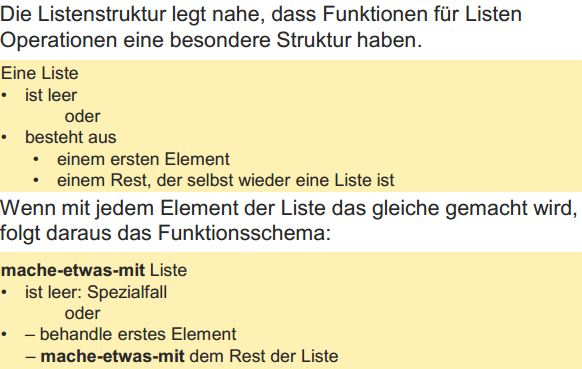
\includegraphics[width=0.7\linewidth]{fig/scheme-recursive-function-schema}
\caption{Verarbeiten von rekursiven Datentypen}
\label{fig:scheme-recursive-function-schema}
\end{figure}

\begin{lstlisting}[caption=Funktionen auf listen]
% Summieren
(define (sum a-list)
	(cond ((empty? a-list) 0)
	(else
	(+ (first a-list) (sum (rest a-list))))))
	
> (sum (list 3 2 1))
6

% Elemente verdoppeln
(define (redouble a-list)
	(if (empty? a-list)
		empty
		(cons
			(* 2 (first a-list)) (redouble (rest a-list)))
))

>(redouble (list 3 2 1))
(list 6 4 2)

% Sortieren von Zahlen
define (insert value a-list)
	(cond
		((empty? a-list) (list value))
		((<= value (first a-list)) (cons value a-list))
		(else (cons (first a-list)
			(insert value (rest a-list))))
))


(define(sort-by-insert num-list)
	(cond
		((empty? num-list) empty)
		(else (insert (first num-list)
			(sort-by-insert (rest num-list))))
))

> (sort-by-insert '(12 54 32 21))
(list 12 21 32 54)
\end{lstlisting}

\subsection{Rekursive Funktionen}
Wenn eine Funktion sich selber aufruft, ist sie rekursiv. Sie beinhaltet eine Verzweigung. Ein Zweig terminiert die Rekursion der andere ruft die Funktion selber wieder auf. Bei \textbf{wohldefinierte Funktionen} terminiert die Auswertung. In den obigen Beispielen wurden strukturelle Rekursionen verwendet. Die Struktur der Funktion folgt nämlich der Struktur der Datenstruktur. Diese sind stets wohldefiniert. 

\section{Funktionen höherer Ordnung}

In der funktionalen Programmierung werden grundsätzlich zwei Arten von Funktionen unterschieden:
\begin{description}
	\item[Funktionen erster Ordnung:] Die Berechnungsmethodik ist fest vorgegeben, nur die Werte der Variablen können unterschiedlich sein.
	\item[Funktionen höherer Ordnung:] Die Berechnungsmethodik sowie die Werte der Variablen können von aussen übergeben werden.
\end{description}
Funktionen sind in Scheme \textit{Werte erster Klasse}, den sie können als Parameter oder Rückgabewert dienen, an Namen gebunden werden und in Listen aufgenommen werden. Funktionen, die andere Funktionen als Parameter und/oder Resultat haben, heissen \textit{Funktionen höherer Ordnung}, bzw. \textit{Higher-Order Functions}. Durch \textit{Funktionen höherer Ordnung} lassen sich komplexe Sachverhalte einfach und kompakt darstellen. In Prolog kann nur \verb|not| als Funktion der booleschen Operatoren übergeben werden. \verb|and| und \verb|or| können nicht als Parameter übergeben werden. Scheme bietet zahlreiche Funktionen (\verb|filter|, \verb|map|, \verb|apply|) an, um effizient mit Listen zu arbeiten.

\subsection{Funktion \texttt{filter}}

Die Funktion \verb|(filter <function> <list>)| wendet \verb|<function>| auf jedes Element von  \verb|<list>| an und liefert eine neue Liste von Elementen zurück, auf die \verb|<function>| zutrifft. \verb|<function>| darf nur ein Argument besitzen (Das jeweilige Element der Liste) und muss einen booleschen Wert zurückliefern (Wenn \verb|true| kommt Element in neue Liste sonst nicht). Listing \ref{lst:funktion-filter} zeigt die Anwendung der \verb|filter|-Funktion mit einem eigenen Prädikat.

\begin{lstlisting}[language=Lisp, caption=Funktion filter, label=lst:funktion-filter]
; Eigene Prädikatsfunktion
(define (squarenumber? value)
	(integer? (sqrt value))
)

> (filter squarenumber? (list 1 2 4 8 16 32 64))
(list 1 4 16 64)
\end{lstlisting}

\subsection{Funktion \texttt{map}}

Die Funktion \verb|(map <function> <list1>…<listN>)| wendet \verb|<function>| auf jedes Element \verb|<list1>…<listN>| an und liefert eine neue Liste zurück. Wenn z.B. zwei Listen (Liste A und B) übergeben werden, wird das erste Element der Liste A und das erste Element der Liste B an \verb|<function>| übergeben und den Rückgabewerte in die neue Liste gespeichert. Danach wird das zweite Element von A und das zweite Element von B übergeben. Deshalb muss \verb|<function>| soviele Argumente besitzen, wie Listen übergeben wurden. Zudem darf \verb|<function>| die Listen nicht verändern. In Listing \ref{lst:funktion-map} wird \verb|map| auf eine bzw. zwei Listen angewendet.

\begin{lstlisting}[language=Lisp, caption=Funktion map, label=lst:funktion-map]
> (map sqr (list 3 5 -6 -23 37 2))
(list 9 25 36 529 1369 4)

> (map + (list 1 2 3) (list 4 5 6))
(list 5 7 9)
\end{lstlisting}

\subsection{Funktion \texttt{apply}}

Die Funktion \verb|(apply <function> <value>…<list>)| nimmt die \verb|<function>| und übergibt \verb|<value>…<list>| als Argumente. Der Aufruf \verb|(apply + 1 -2 3 '(10 20))| ist das selbe wie \verb|(+ 1 -2 3 10 20)|. Als \verb|<value>…<list>| können Werte und/oder Listen übergeben werden. Das letzte Argument muss aber immer eine Liste sein. Natürlich muss \verb|<function>| gleich viele Argumente besitzen, wie es \verb|<value>…<list>| gibt. Listing \ref{lst:funktion-apply} zeigt zwei Anwendungen von \verb|apply|.

\begin{lstlisting}[language=Lisp, caption=Funktion apply, label=lst:funktion-apply]
> (apply / 256 (list 2 4 8))
4 ; 256 wird durch alle Werte geteilt

> (map + (list 1 2 3) (list 4 5 6))
(list 5 7 9)
\end{lstlisting}

Wenn du meinst \verb|map| und \verb|apply| machen eigentlich das selbe, schau mal hier rein\footnote{\href{http://stackoverflow.com/questions/27488723/what-is-the-difference-between-map-and-apply-in-scheme}{http://stackoverflow.com/questions/27488723/what-is-the-difference-between-map-and-apply-in-scheme}} rein.

\section{Anonyme Funktionen}

In Scheme liefert die Auswertung eines Lambda-Ausdrucks eine anonyme Funktion zurück. Ein Lambda-Ausdruck hat folgende Syntax \verb|((lambda (<formal parameters>) <expression>) <argument-list>)|. Die Parameter der Funktion werden beim Ausdruck \verb|<formal parameters>| übergeben. Der Rumpf der Funktion ist der \verb|<expression>|-Teil. Zudem kann eine Liste von Argumenten definiert werden, welche den Parametern zugewiesen werden. Listing \ref{lst:lambda-scope} zeigt, dass ein Parameter welcher in der Lambda-Funktion definiert wurde, nicht von aussen beeinflusst werden kann.

\begin{lstlisting}[language=Lisp, caption=Scope eines Lambda-Ausdrucks, label=lst:lambda-scope]
> (define x 100)
> (define y 200)
> ((lambda (x) (+ x y)) 100) ; Das x oben hat nichts mit diesem x zu tun
300
\end{lstlisting}

Lambda-Ausdrücke sollte man nur verwenden, wenn die Funktion nur einmal gebraucht wird. Sie können deshalb nicht zur Rekursion verwendet werden. Das Wort \textit{Lambda} kommt vom Lambda-Kalkül. Das Lambda-Kalkül besteht aus folgenden drei Bausteinen:
\begin{description}
	\item[Variablen:] Variablen definieren keinen veränderbaren Speicherplatz, sondern sind Variablen im mathematischen Sinne (Platzhalter für konkrete Werte)
	\item[Funktionsabstraktion:]  $\lambda$ x . A definiert eine (anonyme) Funktion, die ein x bekommt, und einen Ausdruck A als Funktionskörper hat (in dem x vorkommen kann, aber nicht vorkommen muss)
	\item[Funktionsapplikation:] F A bedeutet, dass die Funktion F auf den Ausdruck A angewandt wird
\end{description}
Zudem gibt es im Lambda-Kalkül nur Funktionsabstraktionen und Funktionsapplikationen (Es gibt keine Zahlen, Wahrheitswerte, Funktionsnamen usw.). Damit lassen sich dann tolle Sachen machen, die man nicht verstehen muss.

\section{Funktionen mit Gedächtnis}

In der rein funktionalen Programmierung bekommt man für die gleiche Eingabe immer die gleiche Ausgabe einer Funktion. Man kann also den Funktionsaufruf durch seinen Wert ersetzen, ohne den Sinn des Programms zu verändern (z.B. \verb|(+ 3 5)| durch \verb|8| ersetzen). Diese Eigenschaft wird referentielle Transparenz genannt. Funktionen mit Gedächtnis sind nicht mehr rein funktional, weil durch den Zustand Nebeneffekte entstehen können. 

Mit dem Ausdruck \verb|(set! <variable> <expression>)| kann einer Variable ein Wert zugewiesen werden. Dabei muss der Name der \verb|<variable>| definiert sein. Es wird der Ausdruck \verb|<expression>| ausgewertet und der resultierende Wert an den Namen der \verb|<variable>| gebunden. Listing \ref{lst:counter} zeigt einen einfachen Zähler mit Gedächtnis.

\begin{lstlisting}[language=Lisp, caption=Zähler mit Gedächtnis, label=lst:counter]
(define counter-value 0)
(define (increment-counter)
	(set! counter-value (+ 1 counter-value)))
	
> counter-value
0
> (increment-counter)
(void) ; Rückgabewert von set! nicht definiert
> counter-value
1
\end{lstlisting}

Ein weiteres Element der imperativen Programmierung in Scheme ist die Sequenz. Eine Sequenz hat die Form \verb|(begin <expression-1>...<expression-N> <expression>)| und wertet alle \verb|expressions| in der gegebenen Reihenfolge aus. Die Sequenz liefert dann den Wert von \verb|expression| zurück.

\section{Ein- und Ausgabe}

Scheme benutzt Ports für die Ein- und Ausgabe. Ports bedienen Datenquellen oder -senken, z.B. File, Terminal oder TCP Verbindung. Ein Port muss offen sein, bevor man ihn zum Lesen oder Schreiben benutzen kann. Der Standard I/O Port, d.h. der Konsolen I/O-Port, ist beim Start von Scheme automatisch offen. Listing \ref{lst:read-file} zeigt wie man in Scheme eine Datei einliest. 

\begin{lstlisting}[language=Lisp, caption=Datei lesen, label=lst:read-file]
; Port öffnen, um aus der Datei zu lesen
(define in (open-input-file "data.txt"))

(define (read-file a-list)
	; Daten lesen
	(let ((data (read in)))
		(cond
			; Wenn EOF Liste zurückgeben
			((eof-object? data) a-list)
			; Wenn nicht Daten an Liste anhängen und read-file aufrufen
			(else (read-file (cons data a-list)))
		)
	)
)
\end{lstlisting}

Listing \ref{lst:write-file} zeigt wie man eine Liste in eine Datei schreibt. Existiert die Datei bereits wird ein Laufzeitfehler generiert.

\begin{lstlisting}[language=Lisp, caption=Datei schreiben, label=lst:write-file]
; Port öffnen, um in Datei zu schreiben
(define out (open-output-file "output.txt"))

(define (output-file a-list)
	; Wenn Liste leer, Zeilenumbruch schreiben
	(cond ((null? a-list) (newline out))
					 ; Erstes Wort der Liste schreiben
		(else (begin (write (first a-list) out)
					 ; Leerschlag einfügen
					 (write-char #\space out)
					 ; Rest der Liste schreiben
					 (output-file (rest a-list)))
		)
	)
)
\end{lstlisting}

Es sollte nach jeder Schreib- bzw. Leseoperation der Port geflusht und geschlossen werden. In Scheme stehen zahlreiche Bibliotheken für Lese-/Schreib-Funktionen zur Verfügung (z.B. batch-io).